\documentclass[10pt]{article}
\usepackage[a4paper,margin=2cm]{geometry}
\usepackage[T1]{fontenc}
\usepackage{lmodern}
\usepackage{amsmath,amssymb,mathtools}
\usepackage{graphicx}
\usepackage{booktabs}
\usepackage{caption}
\usepackage{parskip}
\captionsetup{font=small,skip=2pt}
\setlength{\parskip}{3pt}
\setlength{\textfloatsep}{6pt}
\setlength{\floatsep}{6pt}
\newcommand{\tr}{\mathrm{Tr}}
\newcommand{\lab}[1]{\noindent\textit{#1}\;}

\title{\vspace{-1.2cm}Pure and Mixed States, State Vectors and Density Matrices\\[2pt]
\large Assignment I report, instance 0986 (fingerprint \texttt{cc999486802f})}
\author{Nihal Krishna Shrivastava (2023B5A70986G) \and Kartik Garg (2023A7PS0397G)}
\date{}

\begin{document}
\maketitle
\vspace{-0.8cm}

\section{States}
Table~\ref{tab:states} lists the single-qubit states of S1 with the purity $\gamma=\tr\rho^2$ and Bloch vector $r_k=\tr(\rho\sigma_k)$ that our code computes. The partly mixed state is $0.8\,|0\rangle\langle0|+0.2\,|1\rangle\langle1|$, built from two states we already had.
\begin{table}[h]
\centering\small
\begin{tabular}{llcc}
\toprule
State & $\rho$ & purity $\gamma$ & Bloch vector $(x,y,z)$\\
\midrule
$|0\rangle$ & $|0\rangle\langle0|$ & 1 & $(0,0,1)$\\
$|+\rangle$ & $|+\rangle\langle+|$ & 1 & $(1,0,0)$\\
$\tfrac12(|0\rangle\langle0|+|1\rangle\langle1|)$ & $I/2$ & 0.5 & $(0,0,0)$\\
$\tfrac12(|+\rangle\langle+|+|-\rangle\langle-|)$ & $I/2$ & 0.5 & $(0,0,0)$\\
partly mixed (0.8/0.2) & $\mathrm{diag}(0.8,0.2)$ & 0.68 & $(0,0,0.6)$\\
\bottomrule
\end{tabular}
\caption{The five single-qubit states of S1. All five pass the validity check (Hermitian, trace 1, eigenvalues $\ge-10^{-10}$).}\label{tab:states}
\end{table}

The two-qubit Bell state $(|00\rangle+|11\rangle)/\sqrt2$ and the three-qubit GHZ state $(|000\rangle+|111\rangle)/\sqrt2$ are pure ($\gamma=1$). Other states in the assignment are outputs of operations: $|+\rangle$ and $|0\rangle$ after each noise channel (S4), the pure output of a 3-qubit, 10-gate circuit (S2: H(0), CX(0,1), RY(0.7) on 2, CX(1,2), T(0), RZ(1.1) on 1, CZ(0,2), H(1), S(2), CX(2,0); see \texttt{s2\_circuit.txt}), and single trajectories with their average (S5, S7).

Our instance is \texttt{0986}: $n=6$ qubits, 14 gates (S, X, H and five CNOTs; the last gate is CNOT(2,5)), dephasing with $p=0.121$ applied after every gate to every qubit the gate touched, bipartition $A=[0,1,2,3,4]$, $B=[5]$, trajectory seed 1103068787. The final state $\rho$ is a noisy 6-qubit mixed state and $\rho_A=\tr_B\rho$ is its 5-qubit reduced state. Qubit 5 is touched only by one S gate and by CNOT(2,5), which is the only gate coupling $B$ to $A$.

\section{Operations}
\lab{O1-O4.} A pure state is $\rho=|\psi\rangle\langle\psi|$ and an ensemble gives $\rho=\sum_ip_i|\psi_i\rangle\langle\psi_i|$. A valid $\rho$ is Hermitian, has trace 1 and is positive semidefinite, which we test with the eigenvalues. Outcome probabilities are $p_m=\langle m|\rho|m\rangle$. For one qubit $\rho=\tfrac12(I+\vec r\cdot\vec\sigma)$, so $\gamma=\tfrac12(1+|\vec r|^2)$. Hence $|\vec r|=\sqrt{2\gamma-1}$: pure states have $|\vec r|=1$ and $I/2$ has $|\vec r|=0$ and $\gamma=\tfrac12$.

\lab{O5, O6.} A unitary acts as $\rho\to U\rho U^\dagger$. For the partial trace we sum over the discarded basis states, $(\rho_A)_{ij}=\sum_k\rho_{(ik),(jk)}$. In Qiskit qubit $q$ of an $n$-qubit state is tensor axis $n-1-q$, and our NumPy routine uses that mapping.

\lab{O7. Channels on the Bloch vector.} Conjugation by a Pauli keeps the component along that Pauli and flips the other two. Therefore
\begin{align*}
\text{bit flip } (X):&\ (x,y,z)\to(x,\,(1-2p)y,\,(1-2p)z),\\
\text{dephasing } (Z):&\ (x,y,z)\to((1-2p)x,\,(1-2p)y,\,z),\\
\text{depolarising}:&\ (x,y,z)\to(1-p)(x,y,z),
\end{align*}
because $(1-p)\rho+p\,\tfrac I2$ shrinks every component by $1-p$. With $\gamma=\tfrac12(1+|\vec r|^2)$ the purities are as follows. For $|+\rangle$ ($\vec r=(1,0,0)$): bit flip gives $1$, dephasing gives $\tfrac12(1+(1-2p)^2)$, depolarising gives $\tfrac12(1+(1-p)^2)$. For $|0\rangle$ ($\vec r=(0,0,1)$): bit flip gives $\tfrac12(1+(1-2p)^2)$, dephasing gives $1$, depolarising gives $\tfrac12(1+(1-p)^2)$.

\lab{O8. Trajectories.} Pick $K_k$ with probability $p_k=\langle\psi|K_k^\dagger K_k|\psi\rangle$ and renormalise. For dephasing this means $Z$ with probability $p$ and $I$ with probability $1-p$. Every trajectory is a pure state $|\psi_i\rangle$ and $\bar\rho_N=\frac1N\sum_i|\psi_i\rangle\langle\psi_i|$ has expectation exactly $\rho$. Since $\tr(|\psi_i\rangle\langle\psi_i|)^2=1$, the mean squared Frobenius distance of one trajectory to $\rho$ is $1-\gamma(\rho)$, and the root-mean-square error of the average is
\begin{equation}
\sqrt{\mathbb E\,\|\bar\rho_N-\rho\|_F^2}=\sqrt{(1-\gamma)/N}\label{eq:err}
\end{equation}
(the mean error is slightly smaller).
Also $\mathbb E\,\gamma(\bar\rho_N)=\gamma+(1-\gamma)/N$, a small upward bias.

\lab{O9. Entropy.} $S(\rho)=-\sum_\lambda\lambda\log_2\lambda$ over the eigenvalues. For a pure bipartite state with Schmidt coefficients $s_i$ the two reduced states share the eigenvalues $s_i^2$, so $S(\rho_A)=S(\rho_B)$, and $S(\rho_B)\le1$ bit when $B$ is a single qubit.

\section{Simulations}
Tolerance: all comparisons use $10^{-10}$. Double precision has relative precision $2\times10^{-16}$ and the matrices here have at most a few thousand entries, so rounding gives errors near $10^{-15}$ (we see $10^{-16}$ to $10^{-15}$ below). A tolerance of $10^{-10}$ keeps five orders of margin for accumulated rounding and still sits far below any physical difference we test, such as the 0.23 gap caused by a wrong qubit order. Trajectory results are statistical, so we compare them with the scale $\sqrt{(1-\gamma)/N}$ instead of $10^{-10}$.

\lab{S1.} Our predictions (in \texttt{predictions.md}; each Before line there was written before the corresponding simulation was run, and each After line afterwards) were purity 1 for $|0\rangle,|+\rangle$, purity 0.5 for both mixtures, and an in-between value for our own state. Results are in Table~\ref{tab:states} and matched; the purity check agrees with the NumPy eigenvalue value to $10^{-10}$. \lab{S2.} We predicted that state-vector and density-matrix routes agree. Five routes (quantum\_info state vector, quantum\_info density matrix, Aer state vector, Aer density matrix, NumPy $U\rho U^\dagger$) give the same $\rho$ within $2.6\times10^{-16}$; the raw state vectors from the two simulators differ by $2.5\times10^{-16}$ with overlap 1. A deliberate qubit reversal changes $\rho$ by 0.23, so the test can detect ordering mistakes. \lab{S3.} Predicted $I/2$ for half a Bell pair. We got $\rho_A=I/2$, $\gamma=0.5$, $S=1$ bit. For GHZ, removing one qubit gives $\mathrm{diag}(0.5,0,0,0.5)$ with $\gamma=0.5$, $S=1$, and removing two gives $I/2$. Qiskit's \texttt{partial\_trace} and our NumPy version agree within $10^{-10}$.

\lab{S4.} Predictions were the formulas of Section 2. The 21-point sweep over $p\in[0,1]$ matches them (Figure~\ref{fig:s4}), and the Aer noise model and the exact Kraus route agree within $4.4\times10^{-16}$ over all 126 cases. \lab{S5.} Predicted pure trajectories and an error that falls like $1/\sqrt N$. Every trajectory was pure. For $|+\rangle$ with dephasing $p=0.3$, 20 repeats per $N$ and seed 2026, the fitted log-log slope is $-0.536$ for Aer and $-0.484$ for our NumPy sampler. \lab{S6.} Predictions: noiseless $S(\rho)=0$ and $S(\rho_A)\le1$; noisy $S(\rho)$ of a few bits and $S(\rho_A)$ within one bit of it, sign unknown. Results are in Table~\ref{tab:s6}. The Aer route and the Kraus route differ by at most $9.7\times10^{-17}$. \lab{S7.} Predicted slope $-0.5$ and a bias $(1-\gamma)/N$ in the purity. We obtained slope $-0.520\pm0.011$ (A3.1). \lab{S8.} Predicted $2^n$ and $4^n$ scaling, and a density-matrix slowdown around $n=4$ or 5. The scaling matched (A3.2) but the slowdown came at $n=10$ to 11, so that part of our prediction was wrong. We took $\texttt{s8\_scaling\_t1}$ (one thread, 3 repeats, median) as our data set.

\begin{table}[h]
\centering\small
\begin{tabular}{lcccc}
\toprule
 & purity $\gamma(\rho)$ & $S(\rho)$ & $S(\rho_A)$ & $S(\rho_B)$\\
\midrule
noiseless & 1 & $6\times10^{-16}$ & 1 & 1\\
dephasing $p=0.121$ & 0.111549021553 & 3.526117392457 & 3.553370440592 & 1\\
\bottomrule
\end{tabular}
\caption{S6 on instance 0986. The purity of $\rho_A$ is 0.5 without noise and 0.1071 with noise.}\label{tab:s6}
\end{table}

\begin{figure}[t]
\centering
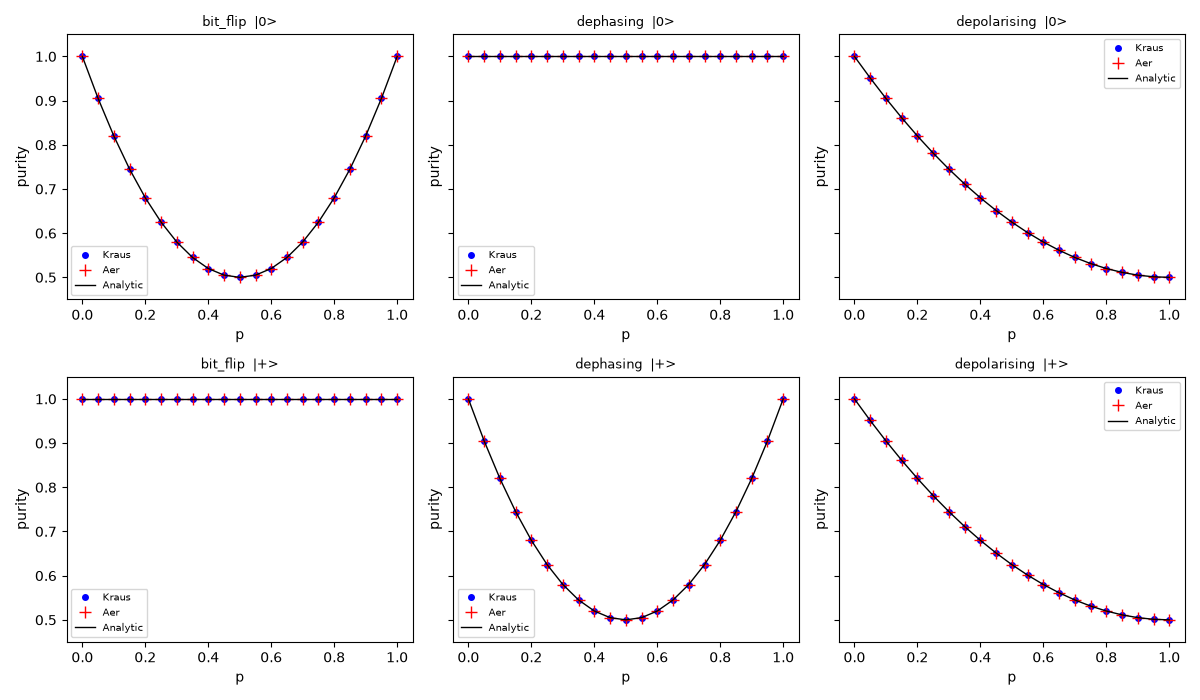
\includegraphics[width=0.82\linewidth]{code/s4_noise_sweep.png}
\caption{S4: purity against $p$ for the three channels on $|0\rangle$ (top) and $|+\rangle$ (bottom). Blue dots are the exact Kraus route, red plus signs the Aer noise model, black lines our hand formulas of Section 2.}\label{fig:s4}
\end{figure}

\section{Analysis}
\subsection*{Level 1}
\lab{Q1.1.} For $|+\rangle$ the $Z$ statistics are $(0.5,0.5)$ and for $\tfrac12(|0\rangle\langle0|+|1\rangle\langle1|)$ they are also $(0.5,0.5)$. In the $X$ basis $|+\rangle$ gives $P(+)=1$, $P(-)=0$, while the mixture gives $(0.5,0.5)$ (our S1 printout). Equivalently $\langle X\rangle=\tr(\rho X)$ is 1 for $|+\rangle$ and 0 for the mixture. The off-diagonal element $\rho_{01}=\tfrac12$ is the coherence between $|0\rangle$ and $|1\rangle$. It leaves the $Z$ statistics alone and sets the $X$ statistics. A mixture only says we do not know which of $|0\rangle,|1\rangle$ we hold, so it has no coherence. A superposition is one definite state whose amplitudes interfere, so it cannot be a mixture. Any mixture of $|0\rangle$ and $|1\rangle$ gives $P(+)=1/2$, so $P(+)=1$ rules every such mixture out.

\lab{Q1.2.} Pure states have $|\vec r|=1$ (on the sphere) and the maximally mixed state has $|\vec r|=0$ (the centre, $\gamma=\tfrac12$). A length in between means a mixed state in the interior of the ball. Our partly mixed state has $|\vec r|=0.6$ and $\gamma=\tfrac12(1+0.36)=0.68$.

\lab{Q1.3.} No. Both mixtures of the third and fourth states give exactly $I/2$ (we printed the matrices and they are identical, purity 0.5, Bloch vector zero). Any orthonormal pair in equal weights gives the same $\rho$, and so do many other ensembles. The density matrix identifies the physical state, since all measurement statistics follow from it, and it keeps no record of which ensemble prepared it. For a non-degenerate $\rho$ such as $\mathrm{diag}(0.8,0.2)$ the eigenvectors give one natural ensemble, yet non-orthogonal ensembles give the same $\rho$; for the degenerate $I/2$ every orthonormal basis works, so the ensemble cannot be recovered.

\subsection*{Level 2}
\lab{Q2.1.} The Bell state has Schmidt decomposition $(|0\rangle_A|0\rangle_B+|1\rangle_A|1\rangle_B)/\sqrt2$ with two equal coefficients. The global state is pure because we know everything about the pair. The information is stored in the correlations between the two qubits (the off-diagonal terms $|00\rangle\langle11|$). Summing over the states of one qubit removes those terms and leaves $\rho_A=\tfrac12(|0\rangle\langle0|+|1\rangle\langle1|)=I/2$, with $\gamma=0.5$ and $S=1$ bit (S3). The qubit alone carries no information about its own state, since all of it lives in the correlation with the partner.

\lab{Q2.2.} Figure~\ref{fig:s4} overlays our formulas on the S4 data and they coincide. Dephasing leaves the purity of $|0\rangle$ unchanged ($\gamma=1$ for every $p$). Bit flip and depolarising reduce it. On the Bloch sphere $|0\rangle$ lies on the $z$ axis. Dephasing conjugates by $Z$, which is a rotation by $\pi$ about $z$ that fixes the axis, so only $x,y$ shrink and $z$ keeps its value. Bit flip is a rotation about $x$ that sends $z\to-z$, so with probability $p$ the vector points the other way and the average $z$ becomes $1-2p$. Depolarising shrinks all components. The roles swap for $|+\rangle$, which lies on the $x$ axis: bit flip leaves it unchanged and dephasing shrinks it. The bit flip curve on $|0\rangle$ and the dephasing curve on $|+\rangle$ return to 1 at $p=1$ because a full flip is a unitary, and they reach 0.5 at $p=0.5$. Depolarising only reaches 0.5 at $p=1$ in the O7 convention.

\lab{Q2.3.} A single trajectory is a pure state because one Kraus operator is applied and the vector is renormalised. For $|+\rangle$ with dephasing the trajectory is $|+\rangle$ (probability $1-p$) or $|-\rangle$ (probability $p$). The mixedness lives in the ensemble. The average $\bar\rho_N$ is $\tfrac12\begin{psmallmatrix}1&1-2k/N\\1-2k/N&1\end{psmallmatrix}$, where $k$ is the number of $Z$ events, and tends to $\rho$ with off-diagonal entry $\tfrac12(1-2p)$. So the mixedness of $\rho$ is our ignorance of which trajectory occurred. In S5 (Aer shot = one trajectory) the mean error dropped from 0.170 at $N=10$ to 0.0032 at $N=30000$, a factor 53, while $\sqrt{3000}=55$. The log-log slopes are $-0.536$ (Aer) and $-0.484$ (NumPy), close to $-0.5$, and both sit near the curve $2\sqrt{p(1-p)/(\pi N)}$. The average of pure states also has purity slightly above the exact value, by about $(1-\gamma)/N$.

\lab{Q2.4.} \texttt{pauli\_error([('X',p),('I',1-p)])} and the $Z$ version take the probability $p$ directly, so they equal O7 with no conversion. \texttt{depolarizing\_error($\lambda$,1)} acts as $\rho\to(1-\lambda)\rho+\lambda I/2$, so $\lambda=p$ in O7 (its allowed range extends to $4/3$, which we do not use). We checked at $p=0.3$: the \texttt{SuperOp} of Qiskit's error and of our Kraus channel differ by $1.3\times10^{-15}$. The tempting wrong guess is $X,Y,Z$ each with probability $p/3$, which shrinks the Bloch vector by $1-4p/3$ and is a different channel. At $p=0.3$, \texttt{depolarizing\_error(0.3, 1)} maps $|+\rangle$ to Bloch vector $(0.7,0,0)$, purity 0.745, while putting $p/3$ on each Pauli gives $(0.6,0,0)$, purity 0.68. The convention that caught us out was qubit ordering. Qiskit is little-endian, so the bitstring \texttt{q2 q1 q0} puts qubit 0 on the right, and tracing out qubit $q$ in NumPy needs axis $n-1-q$. A reversed ordering in S2 gives a $\rho$ off by 0.23. A second trap was in S4: \texttt{transpile()} removes \texttt{id} gates, and the \texttt{id} gate carried the noise, so the noise was silently dropped until we sent the circuit to Aer unchanged.

\subsection*{Level 3}
\lab{A3.1.} Figure~\ref{fig:l3} shows the S7 error $\|\bar\rho_N-\rho\|_F$ against $N$ on log-log axes, from $N=16$ to 8192, using the exact $\rho$ from S6 and 8192 stored trajectories split into blocks. The error falls from 0.231 at $N=16$ to 0.0100 at $N=8192$ and the fitted slope is $-0.520\pm0.011$ (standard error of the fit), close to $-0.5$. The curve follows Eq.~\eqref{eq:err}, which gives 0.236 and 0.0104 at the two ends with $1-\gamma=0.8885$. At $N=8192$ the trajectory purity is 0.111427 against exact 0.111549, a difference of $-1.2\times10^{-4}$. This is smaller than the statistical scatter of about $1.6\times10^{-3}$, and the expected bias $(1-\gamma)/N=1.1\times10^{-4}$ is below it, so it cannot be seen. The run took 234\,$\mu$s per trajectory.

\begin{figure}[t]
\centering
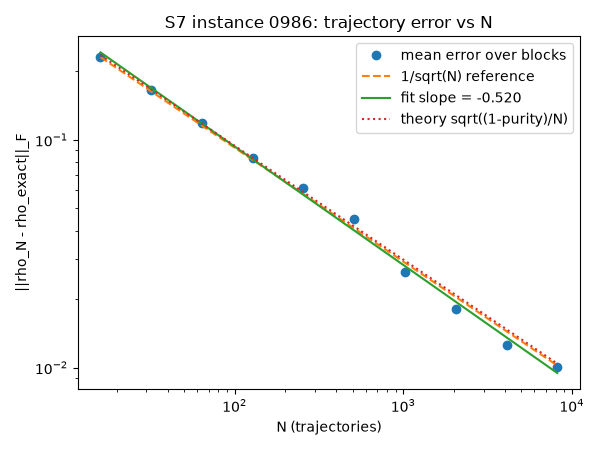
\includegraphics[width=0.5\linewidth]{code/s7_traj_error.png}
\caption{S7 error against $N$ (log-log) with the $1/\sqrt N$ guide, the fit and Eq.~\eqref{eq:err}.}\label{fig:l3}
\end{figure}

\begin{figure}[t]
\centering
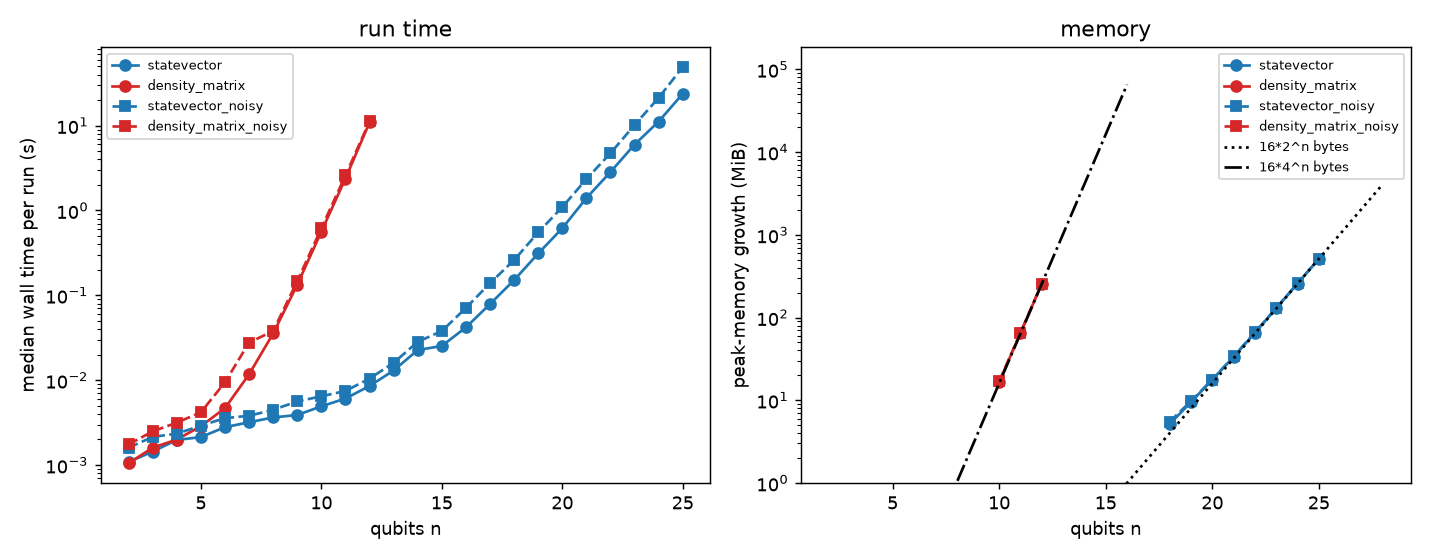
\includegraphics[width=\textwidth]{code/s8_scaling_t1.png}
\caption{Left: run time; right: peak memory; state vector (blue) and density matrix (red). One thread, median of 3 runs; solid lines noiseless, dashed lines noisy.}\label{fig:s8}
\end{figure}

\lab{A3.2.} From the one-thread S8 data (Figure~\ref{fig:s8}; depth-10 circuit family, wall-clock median of 3 runs), the fitted log$_2$ slopes of time against $n$ are $+1.04$ for the state vector (fit over $n=18$ to 25) and $+2.11$ for the density matrix ($n=9$ to 12), against 1 and 2 from $2^n$ and $4^n$. The memory slopes are $+0.95$ and $+1.97$, and at the largest sizes the measured peak growth is within 0.6\% of the state size $16\cdot2^n$ and $16\cdot4^n$ bytes. In the noiseless family the density matrix reached 10.9 s and 256 MiB at $n=12$, where its ladder ended. The noiseless state vector took 1.4 s at $n=21$ and 23.8 s with 512 MiB at $n=25$. At $n=12$ the noiseless state vector needs 8.5 ms, so the density matrix is 1280 times slower and 4096 times larger there. Overhead: at $n=2$ both methods take about 1.1 ms per run, and the state-vector time stays below 4 ms up to $n=8$, so small sizes are dominated by a fixed per-call cost and show no exponential growth yet. Aer's internal timer and our wall clock agree within about 1\% for $n\ge14$ and both show about 1 ms at $n=2$, so this cost sits inside Aer's call path and our timing code adds little. At small $n$ the memory growth is 0.1 to 0.6 MiB, far above the 0.06 MiB or less that the state needs, which is allocator and runtime overhead.

\lab{A3.3.} Assumptions: the cost of one trajectory is the single-shot noisy state-vector time from S8, the density-matrix cost is the noisy density-matrix time, both with the same circuit family; the number of trajectories for Frobenius error $\varepsilon$ is $N=(1-\gamma)/\varepsilon^2$ from Eq.~\eqref{eq:err}, with $1-\gamma\approx0.9$ (our instance has 0.89 and 1 is the upper bound); we want the full $\rho$ up to error $\varepsilon$. We assume the goal is a few observables or the purity; rebuilding the full $\bar\rho_N$ costs $4^n$ memory per trajectory, which removes the memory advantage. Trajectories are cheaper when $N\,t_{SV}(n)<t_{DM}(n)$. The measured ratio $t_{DM}/t_{SV}$ is 2.6, 7.3, 8.5, 26, 96, 347 and 1073 for $n=6,\dots,12$. The crossover sizes are:
\begin{center}\small
\begin{tabular}{cccc}
\toprule
$\varepsilon$ & $N$ & crossover $n$ & basis\\
\midrule
0.3 & 10 & 9 & measured\\
0.1 & 90 & 10 & measured\\
0.03 & 1000 & 12 & measured\\
0.01 & 9000 & 14 to 16 & extrapolated, ratio grows 2 to 3.7 per qubit\\
\bottomrule
\end{tabular}
\end{center}
At $n=15$ the density matrix would need 16 GiB, more than the 7.4 GiB of our machine, so the last row cannot be run here and is an extrapolation. Higher accuracy needs more trajectories ($N\propto\varepsilon^{-2}$), which moves the crossover to larger $n$ by between $\log_2(1/\varepsilon)$ and $2\log_2(1/\varepsilon)$ qubits, since the ratio grows by a factor of 2 to 3.7 per qubit. For $n\le6$ the density matrix wins at every accuracy we consider.

\lab{Q3.1.} For our instance $S(\rho_A)=3.5534>S(\rho)=3.5261$, by 0.027 bit, so $\rho_A$ is slightly more mixed than $\rho$. Without noise it is $1>0$. The conditional entropy $S(B|A)=S(\rho)-S(\rho_A)=-0.027<0$ is negative, which a separable state cannot have, so $A$ and $B$ are still entangled, although only just. The mutual information $S(A)+S(B)-S(AB)$ is 1.027 bits, down from 2 bits without noise, so dephasing removed about half of the $A$-$B$ correlation. For a pure global state $S(\rho_A)\ge S(\rho)=0$ always, so this ordering is possible, and it is what we see without noise. For a mixed state, $S(\rho_A)>S(\rho)$ is enough to show entanglement (it means $S(B|A)<0$), though entangled mixed states can also have $S(\rho_A)<S(\rho)$. In our instance the noise shrinks the gap from 1 bit to 0.027 bit.

\lab{Q3.2.} Classical uncertainty is mixedness from not knowing which pure state or noise event occurred. Entanglement-induced mixedness appears when a pure global state is viewed through one part. In our results, the first shows up in the noisy instance: the global entropy $S(\rho)=3.53$ bits (purity 0.1115) for a 6-qubit state that was pure before the dephasing, and also in the S5 ensemble of $|+\rangle,|-\rangle$. The second shows up in the noiseless instance: $S(\rho)=0$ yet $S(\rho_A)=1$ bit, and in the Bell state $\rho_A=I/2$ from a pure $\rho$. The two combine in the noisy instance, where $S(\rho_A)=3.55$ includes both effects.

\lab{Q3.3.} Trajectories win at $n=12$ (noisy circuit family): one trajectory takes 10.4 ms and the density matrix 11.2 s, so up to about 1000 trajectories ($\varepsilon\approx0.03$) are cheaper, and trajectories also reach $n=25$ in 49 s and 512 MiB, where the density matrix would need about 16 PiB. Density matrices win at small $n$ and when exactness is wanted. For the instance ($n=6$) the exact route gives purity and entropies to $10^{-16}$, while 8192 trajectories take about 1.9 s and still differ by $10^{-4}$ in purity. In the S8 family at $n=6$ the density matrix takes 9.4 ms and a single trajectory already costs 3.6 ms, so 90 trajectories would cost about 35 times more. We separate the two as follows. Algorithmically a trajectory costs $\propto2^n$ per gate and the density matrix $\propto4^n$, and the number of trajectories $N$ depends on $\varepsilon$ and $1-\gamma$ but not on $n$, so the ratio doubles per qubit asymptotically. The simulator adds a fixed per-call cost near 1 to 2 ms. It makes the ratio close to 1 for $n\le5$ (1.1 to 1.4), which is why our predicted slowdown at $n=4$ to 5 failed to appear. From $n=9$ to 12 the ratio rises by 3.1 to 3.7 per qubit, faster than 2, because the state-vector time (5.6 to 10.4 ms) is still near the overhead floor while the density matrix has already left it. The same overhead is amortised in batches: S7 shows 234\,$\mu$s per trajectory at $n=6$ for 8192 shots in one call against 3.6 ms for a single-shot call, so the best trajectory timings come from batching many shots.
\end{document}
